\documentclass{beamer}
\usepackage[slovene]{babel}
\usepackage[utf8]{inputenc}
\usepackage[T1]{fontenc}

\usepackage{amsmath}
\usepackage{amsthm}
\usepackage{amsfonts}
\usepackage{url}
\usepackage{graphicx}
\usepackage{enumerate}
\usepackage{listings}
\graphicspath{ {images/} }
 
 
%Information to be included in the title page:
\title{VS postopek za izračun vrednosti polinomov več spremenljivk}
\author{Janez Radešček, Miha Avsec}
\institute{Fakulteta za matematiko in fiziko}
\date{2019}
 
 
 
\begin{document}
 
\frame{\titlepage}

\begin{frame}
\frametitle{Polinom v Bezierjevi obliki}

$$p(r,s,t) = \sum_{i=0}^{d}\sum_{j=0}^{i}b_{d-i,i-j,j}B_{d-i,i-j,j}^{d},$$
kjer je
$$B_{i,j,k}^{d}(r,s,t) = \frac{d!}{i!j!k!}r^is^jt^k.$$

\end{frame}

\begin{frame}
\frametitle{decasteljou}



\end{frame}



\begin{frame}
\frametitle{MBB oblika}

$$p(r,s,t) = \sum_{i=0}^{d}\sum_{j=0}^{i}c_{d-i,i-j,j}r^{d-i}s^{i-j}t^j,$$
tako da za koeficiente $c_{d-i,i-j,j}$ vzamemo
$$c_{d-i,i-j,j} = \frac{d!}{(d-i)!(i-j)!j!}b_{d-i,i-j,j}, \quad j=0,\ldots, i; i = 0,\ldots,d.$$
\end{frame}


\begin{frame}
\frametitle{MBB oblika}
\begin{center}
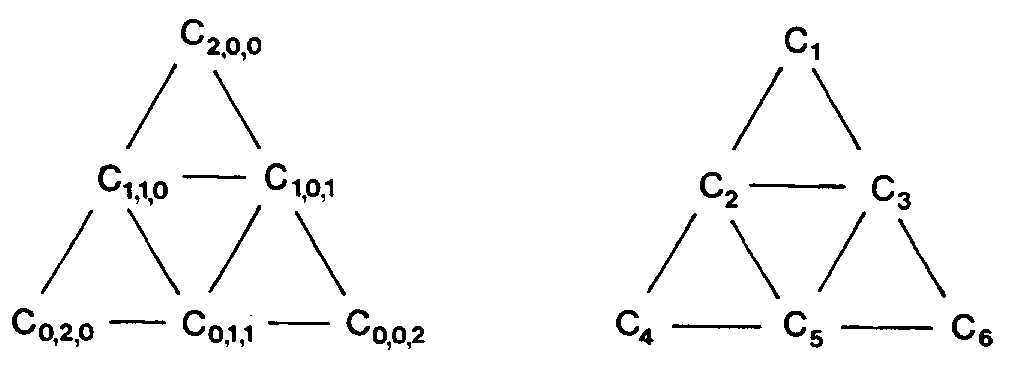
\includegraphics[width=.9\linewidth]{graf.png}
\end{center}

\end{frame}

\begin{frame}
\frametitle{algoritm MBB}
\end{frame}

\begin{frame}
\frametitle{Taylor}
$$p(u,v) = \sum_{i = 0}^n{\sum_{j=0}^{n-i}{a_{i,j}u^iv^j }}$$
\end{frame}



\begin{frame}
\frametitle{algoritem}
\end{frame}

\begin{frame}
\frametitle{tabelca}
\end{frame}


\begin{frame}
\frametitle{tetraeder}
\end{frame}































\end{document}